\chapter{Attack Model}\label{ch:attack}

In this chapter, we will extensively present the threat model of BREACH. We will
explain the conditions that should be met in order for the attack to be
launched and describe our implementation for the attack. We will also
investigate the types of vulnerabilities in web applications that can be
exploited with this attack, as well as introduce alternative types of exploits
that have not been presented before.

\section{Mode of Operation}\label{sec:mo}

This section provides the model of the attack, the conditions that are required
for the attack to launch and the implementation that was developed for the
purpose of this work.

\subsection{Description}

The first step is for the attacker to gain control of the victim's network.
Specifically, the attacker needs to be able to view the victim's encrypted
traffic, which can be accomplished using the Man-in-the-Middle techniques
described in Section \ref{sec:mitm}.

After that, the script that issues the requests needs to be executed from the
victim's browser. One way to do this is to persuade the victim to visit a
website controlled by the attacker. This is usually possible with social
engineering methods.

The script issues multiple requests on the target endpoint which are sniffed by
the attacker. As described in Section \ref{sec:sameorigin}, the attacker cannot
read the plaintext of a response, although the lengths of both the request and
the response is visible on the network.

Each request contains a chosen stream of data that gets reflected in the
response. Since the victim is logged in the targeted endpoint website, the
response body will also contain the secrets. If the conditions defined in
Section \ref{subsec:lz77} are met, the secret and the reflection will be
compressed and encrypted.

By issuing a large amount of requests for different inputs the attacker can
analyse the response lengths and extract information about the secrets when a
response presents different length behaviour than the rest.

\subsection{Man-in-the-Middle implementation}

In order to gain control of the victim's traffic toward a chosen endpoint, we
created a Python script that acts as a Man-in-the-Middle proxy.

The IPs and ports of the victim and the endpoint are configured in the
constants' file and the Python script opens connections over TCP sockets on
both directions so that traffic from the victim to the endpoint and vice versa
is routed through the Man-in-the-Middle proxy.

After the environment is set, the script waits for a packet to be received on
either of the sockets, at which point the source of the packet is identified and
the data is parsed in order to log the TLS header and the payload. Eventually,
the packet is forwarded to the appropriate destination.

The parsing of the packet data is essential, since the header contains
information regarding the version of TLS used as well as the length of the
record.

Trying to spot a fragmented record payload, the length of the packet payload is
compared to the length defined in the TLS header. In case the packet is smaller
than the length declared in the header, the number of remaining bytes is stored,
so that these bytes will be taken into account when following packets of same
origin are received. In case the TLS header is fragmented, which can be deduced
when the total bytes of the packet are less than 5, the actual data fragment
needs to be stored so that, combined with the following packet, it can be
translated to a valid TLS record.

Finally, a TLS downgrade attack mechanism is also implemented. In order to test
whether a TLS downgrade attack is feasible, the \texttt{client hello} packet is
intercepted and dropped while the mitm sends a fatal \texttt{handshake failure}
alert response to the victim. The victim's browser is usually configured to
attempt a connection with a lower TLS version where it should also include the
\texttt{tls\_fallback\_scsv} option in the cipher suite list. If the server is
configured properly, the downgrade attempt should be recognised by the
\texttt{tls\_fallback\_scsv} pseudo-cipher and the connection should be dropped.
In other case, the TLS version could be downgraded to a point where a less safe
connection is established such as SSL 3.0 or using the RC4 stream cipher.

A log from a downgrade attempt against Facebook touch, that was created by our
MitM proxy, can be found in Appendix section \ref{sec:downgrade_log}. For
further information on the downgrade vulnerability see the POODLE attack
\cite{poodle}.

The code of the Man-in-the-Middle proxy, as well as the constants' file, can
be found in Appendix sections \ref{sec:connect_py} and \ref{sec:constants_py}.

\subsection{BREACH Javascript implementation}

For the implementation of the BREACH Javascript, we assume the user has provided
the alphabet that the characters of the secret belong to as well as the known
prefix needed to bootstrap the attack. This information will be written to a
file used by the script that performs the attack, an example of which is shown
below:

\plaintext{file with request parameters.}{serial_request.txt}

The script uses the jquery
library\footnote{\url{http://code.jquery.com/jquery-2.1.4.min.js}} to read the
information from the file and issue the attack. If the file is corrupt or either
of the attack variables has changed, a delay of 10 seconds is introduced, until
the system is balanced. After that, serial requests for each item of the attack
vector are made, continuing from the beginning when the end of the vector is
reached.

A delay of 10 seconds is also introduced if the above function fails for any
reason, i.e. if the information file does not exist. That way the attack is
persistent and it is the framework's responsibility to provide the script with a
valid information parameters' file.

For the purpose of this work, the script was included in a local minimal HTML
web page that was visited in order for the attack to begin. However, with slight
modifications it could be run on real world applications or be injected in HTTP
responses, as described in the following section.

The BREACH script and the HTML web page can be found in the Appendix sections
\ref{sec:evil_js} and \ref{sec:index_html}.

\subsection{Attack persistence}\label{sec:persistence}

In this section we will propose a \texttt{command-and-control} mechanism that
makes the attack much more practical. Specifically, we will describe how the
attack can be implemented even if the victim does not visit a contaminated web
page but simply browses the HTTP web.

Since the attacker controls the victim's network, it is possible to inject the
attack script in a response from a regular HTTP website. The script will then
run on the victim's browser, as if the script was part of the HTTP web page all
along.

The following figure depicts this methodology, which is based on the fact that
regular HTTP traffic is not encrypted and also does not ensure data integrity.

\begin{figure}[h] \caption{Command-and-control mechanism} \centering
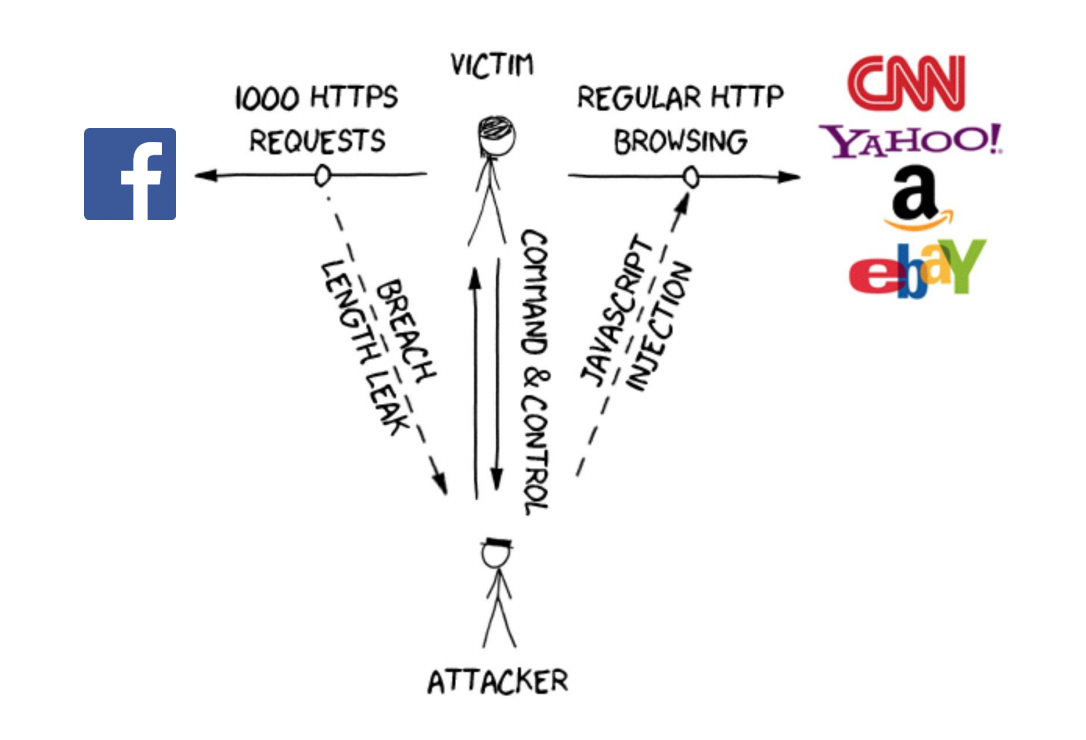
\includegraphics[width=0.6\textwidth]{diagrams/breach_mitm.png}\end{figure}

It is clear that even if the victim stops the connection with the specific HTTP
website, the script can be injected in the next HTTP website that is requested,
resuming the attack session from where it was stopped.

\section{Vulnerable endpoints}\label{sec:vulnerabilities}

In the original BREACH paper \cite{breach}, Gluck, Harris and Prado investigated
the use of CSRF tokens included in HTTP responses as secrets to be stolen.
In this work we suggest alternative secrets as well as point out specific
vulnerabilities on widely used web applications, such as Facebook and Gmail.

\subsection{Facebook Chat messages}\label{subsec:fb}

Facebook is the biggest social network as of 2015 with millions of people using
its chat functionality to communicate. The mobile version, Facebook
Touch\footnote{\url{https://touch.facebook.com}} provides a lightweight
alternative for faster browsing. In this work we present a vulnerability
that allows an attacker to steal chat messages from Facebook Touch, using the
BREACH attack.

Mobile versions of websites provide a good alternative compared to full versions
for a list of reasons. Firstly, these endpoints provide limited noise, given
that they provide a lighter user interface compared to full versions.  Noise
can be defined as any kind of string that changes between requests, such as
timestamps or tokens, which consequently affects the length of the
compressed HTML code even for the same request URL. Secondly, given that the
plaintext is smaller in mobile versions, the possibility of the text that
exists between the secret and the reflection to be larger than the window of
the LZ77 compression is reduced.

Facebook has launched a mechanism to prevent the original BREACH attack against
CSRF
tokens\footnote{\url{https://www.facebook.com/notes/protect-the-graph/preventing-a-breach-attack/1455331811373632?_rdr=p}}.
However, as of August 2015, it has not created a mitigation technique against
the same attack on private messages. An attack method that could steal such
messages is described in the following paragraphs.

Facebook Touch provides a search functionality via URL, where one can search for
messages or friends. Specifically, when a request is made for
\url{https://touch.facebook.com/messages?q=}<search\_string>, the response
contains the chat search results for the given search string. If no match is
found, the response consists of an empty search result page. However, this page
also contains the last message of the 5 latest conversations, which can be seen
in the top drop-down message button of the Facebook user interface, as depicted
below:

\begin{figure}[h] \caption{Facebook Chat drop-down list} \centering
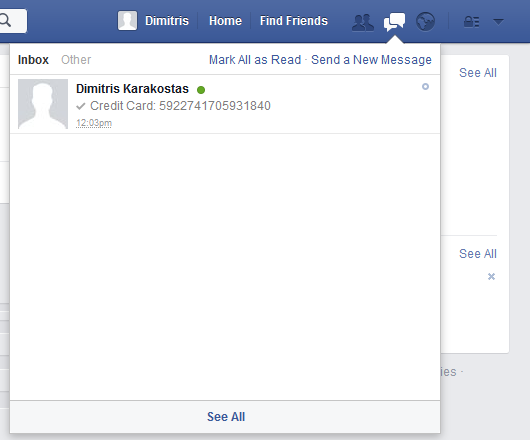
\includegraphics[width=0.6\textwidth]{diagrams/fb_message.png}\end{figure}

The next step is to validate that the search string is reflected in the
response, which should also contain the private secret. Below is a fragment of
the HTML response body, where it can be clearly seen that this condition is met:

\begin{figure}[h] \caption{Facebook response body containing both secret and
reflection} \centering
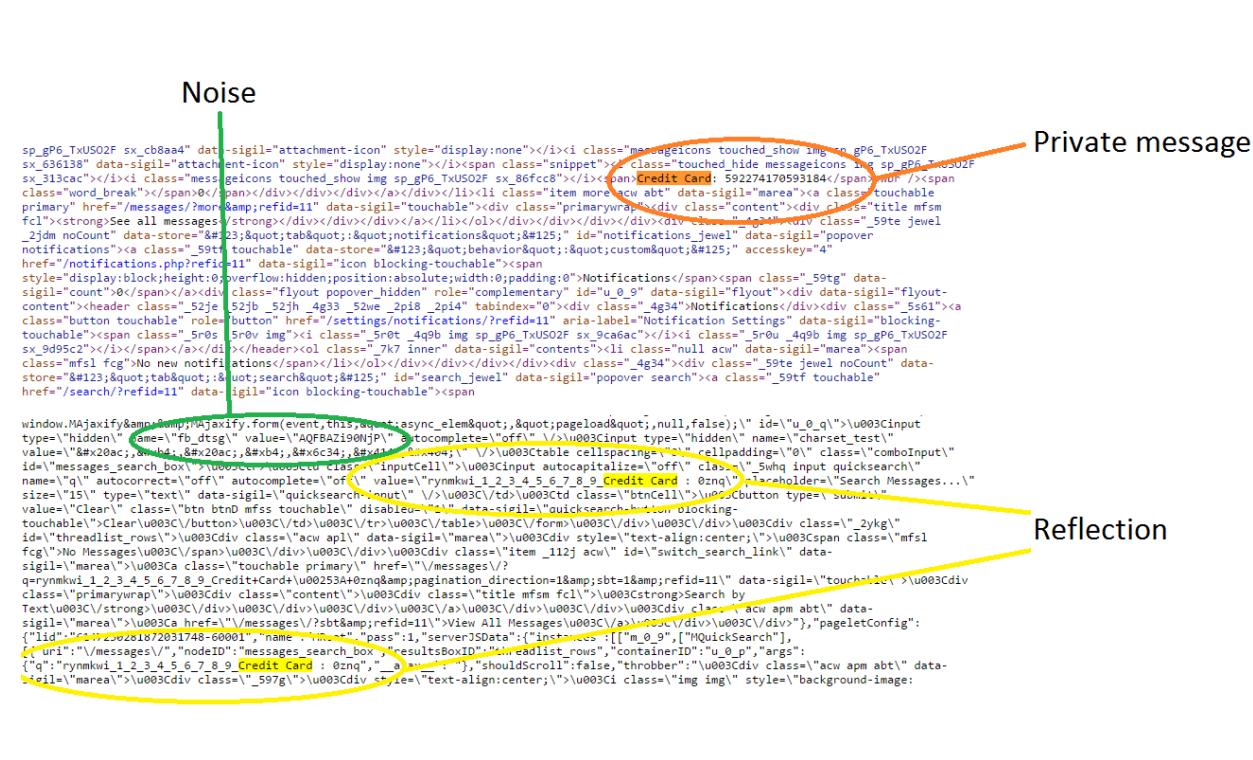
\includegraphics[width=1.1\textwidth]{diagrams/fb_response.png}\end{figure}

If the search string was not reflected in the response the attack could still
be feasible, as long as the attacker could send private messages to the victim.
In that case the private messages from the attacker would be included in the
latest conversations list along with the secret messages from third friends of
the victim, resulting in the compression between the two and thus the partially
chosen plaintext attack.

So, at this point, one of the basic assumptions of the attack, the fact that a
secret and an attacker input string should both be contained in the response,
has been confirmed, providing us with a vulnerability that can be exploited in
the context of the attack.

\subsection{Gmail authentication token}\label{subsec:gmail_token}

Gmail is one of the most used and trusted mail clients as of 2015. It also
provides a plain HTML version for faster, lightweight
interaction\footnote{\url{https://m.gmail.com}}. Gmail uses an authentication
token, which is a random string of digits, letters (uppercase and lowercase) and
dashes, generated every time the user logs in the account.

Opposed to Facebook, Google has not issued any mechanism to mask the
authentication token for different user sessions, but instead uses the same
token for a large amount of requests. This functionality could possibly result
to a threat against the confidentiality of the account.

Requests on \url{m.gmail.com} redirect to another directory of the full website,
specifically \url{https://mail.google.com/mail/u/0/x/}<random\_string>, where
the random string is generated for every request and can be used only for the
particular session.

Gmail also provides a search via URL functionality, similar to the one described
for Facebook Touch. Specifically, a user can search for mails using a URL such
as \url{https://mail.google.com/mail/u/0/x/?s=q&q=}<search\_string>. If no
valid string is provided in the place where the random string is supposed
to be, Google will redirect the request to a URL where the vacation will be
filled with a randomly generated string and return an empty result page,
stating the search action as incomplete, as shown below:

\begin{figure}[h] \caption{Invalid Gmail search} \centering
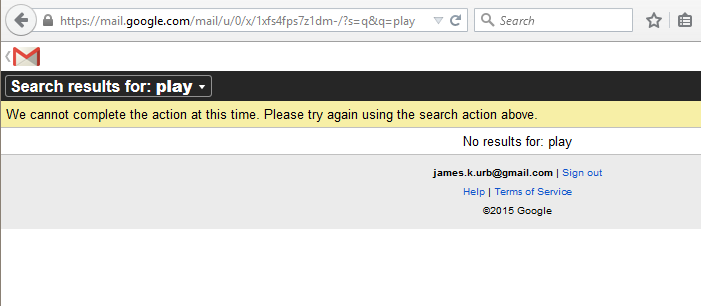
\includegraphics[width=1\textwidth]{diagrams/gmail_search.png}\end{figure}

However, the HTML body of the response contains both the search string and the
authentication token, as can be seen in the following figure:

\begin{figure}[h] \caption{Gmail response body containing both secret and
reflection} \centering
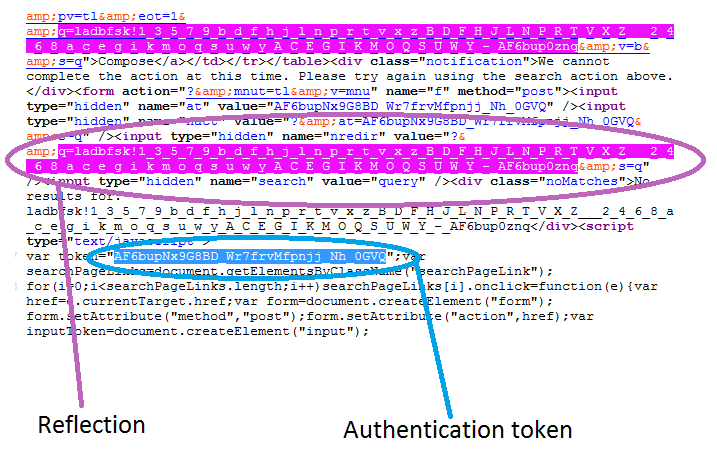
\includegraphics[width=1\textwidth]{diagrams/gmail_response.png}\end{figure}

Another vulnerability that can be exploited is when trying to find the first
three characters to bootstrap the attack. In the response body, the
authentication token is included as below:

\begin{figure}[h] \caption{Gmail authentication token} \centering
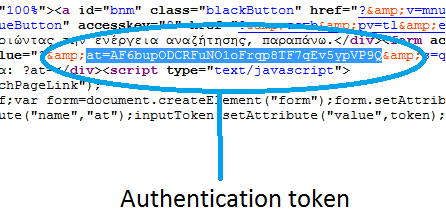
\includegraphics[width=0.6\textwidth]{diagrams/gmail_bootstrap.png}\end{figure}

The authentication token is preceded by the characters \texttt{at=}, which can
be used as the initiating prefix of the attack. Furthermore, the prefix
\texttt{AF6bup} of the token is static, regardless of the session and the
account used. This prefix can also be used in a similar manner to bootstrap the
attack.

\subsection{Gmail private emails}\label{subsec:gmail_mail}

Another opportunity for attack is provided by the search functionality of the
full gmail website. If a user issues a search request in a URL like
\url{https://mail.google.com/mail/u/0#search/}<search\_string> and the search
response is empty, the HTML body will also contain both the subject and an
initial fragment of the body of the latest inbox mails:

\begin{figure}[h] \caption{Gmail empty search response containing latest mails}
\centering
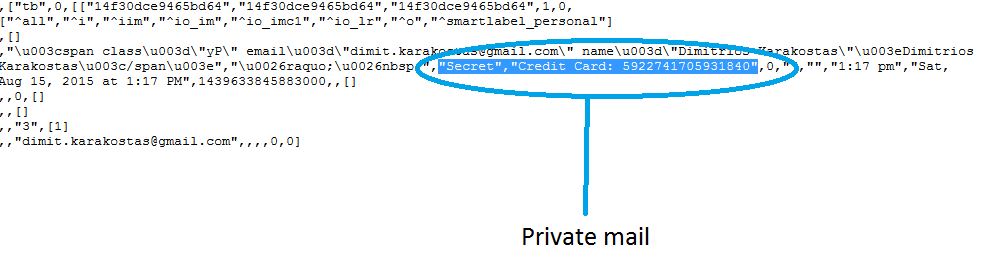
\includegraphics[width=1.1\textwidth]{diagrams/gmail_plain_response.png}\end{figure}

Although in that case the response body does not include the search string, an
attacker could send multiple mails to the victim, which would be included in the
response along with other new messages. That way the attacker could insert a
chosen plaintext in the HTML body and configure the attack under that context.

The above vulnerability shows that secrets and attacker input cannot always be
distinguished. In this case both the secret and the input are emails
making the mitigation of the attack particularly hard.

\section{Validation of secret-reflection compression}\label{sec:mitmproxy}

In previous sections, we have found multiple vulnerabilities on known websites.
We have confirmed that the attacker's chosen plaintext and the secret are both
contained in the HTML response body. In this section, we will present a
methodology to confirm that the chosen plaintext and the secret are also
compressed well when the plaintext matches the secret and badly in any other
case.

The first tool used is mitmproxy\footnote{\url{https://mitmproxy.org}}.
Mitmproxy is described as "an interactive console program that allows traffic
flows to be intercepted, inspected, modified and replayed". For the purposes of
our work, mitmproxy was used to extract the compressed HTML body of two search
request, in the Facebook context described in section \ref{subsec:fb}. The first
search string contained a selected prefix followed by an incorrect character,
while the second contained the same prefix followed by the correct character of
the secret.

The second tool used is infgen\footnote{\url{http://www.zlib.net/infgen.c.gz}}.
infgen is a disassembler that gets a gzip stream as input and outputs the
Huffman tables and the LZ77 compression of the initial data stream.

Applying infgen on the two HTML responses we obtained with mitmproxy, the
comparison between the correct and the incorrect search string can be seen in
the following figure:

\begin{figure}[h] \caption{Comparison of two compressed responses}
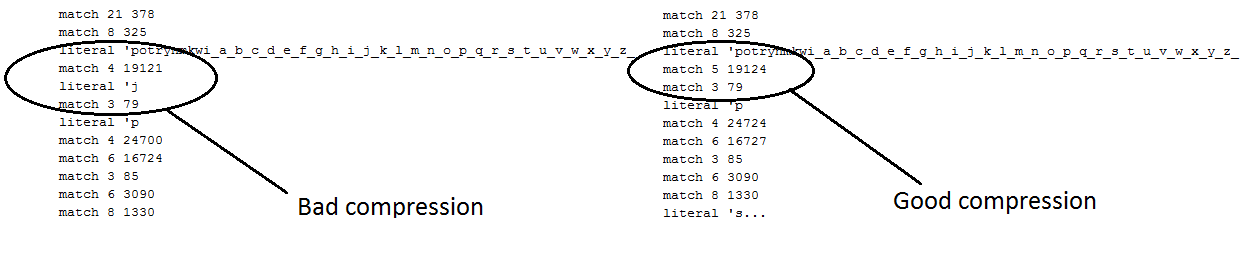
\includegraphics[width=1.15\textwidth]{diagrams/compression_comparison.png}\end{figure}

The left part of the figure shows the compression when the incorrect character
is used. In that case, the prefix is matched so 4 characters are compressed,
while the next character is not compressed and is included as a literal instead.

The right part shows the correct character compression, in which case both the
prefix and the character are compressed, resulting in 5 total characters to be
included in the reference statement and no literal statement.

It is understood that in the second case, since the compression is better the
LZ77 compressed text is smaller, possibly resulting to the final encrypted text
being smaller.

The above described methodology can be used in general in order to test whether
a website compresses two portions of text and to verify that the conditions of a
PCPA attack are met.
